%%%%%%%%%%%%%%%%%%%%%%%%%%%%%%%%%%%%%%%%%
% a0poster Portrait Poster
% LaTeX Template
% Version 1.0 (22/06/13)
%
% The a0poster class was created by:
% Gerlinde Kettl and Matthias Weiser (tex@kettl.de)
% 
% This template has been downloaded from:
% http://www.LaTeXTemplates.com
%
% License:
% CC BY-NC-SA 3.0 (http://creativecommons.org/licenses/by-nc-sa/3.0/)
%
%%%%%%%%%%%%%%%%%%%%%%%%%%%%%%%%%%%%%%%%%

%----------------------------------------------------------------------------------------
%	PACKAGES AND OTHER DOCUMENT CONFIGURATIONS
%----------------------------------------------------------------------------------------

\documentclass[a0,portrait]{poster}

\usepackage{multicol} % This is so we can have multiple columns of text side-by-side
\columnsep=100pt % This is the amount of white space between the columns in the poster
\columnseprule=3pt % This is the thickness of the black line between the columns in the poster

\usepackage[svgnames]{xcolor} % Specify colors by their 'svgnames', for a full list of all colors available see here: http://www.latextemplates.com/svgnames-colors

\usepackage{times} % Use the times font
%\usepackage{palatino} % Uncomment to use the Palatino font

\usepackage{graphicx} % Required for including images
\usepackage{booktabs} % Top and bottom rules for table
\usepackage[font=small,labelfont=bf]{caption} % Required for specifying captions to tables and figures
\usepackage{amsfonts, amsmath, amsthm, amssymb} % For math fonts, symbols and environments
\usepackage{wrapfig} % Allows wrapping text around tables and figures

\begin{document}

%----------------------------------------------------------------------------------------
%	POSTER HEADER 
%----------------------------------------------------------------------------------------

% The header is divided into two boxes:
% The first is 75% wide and houses the title, subtitle, names, university/organization and contact information
% The second is 25% wide and houses a logo for your university/organization or a photo of you
% The widths of these boxes can be easily edited to accommodate your content as you see fit

\begin{minipage}[b]{0.6\linewidth}
\veryHuge \color{NavyBlue} \textbf{NDNCERT in Identity Manager} \color{Black}\\ % Title
\Huge\textit{Implementing an NDN identity manager on Android}\\[2cm] % Subtitle
\Large \textbf{Yuyang(Peter) Rong, Arthi Padmanabhan, Lixia Zhang \footnotemark}\\[0.5cm] % Author(s)
\Large ShanghaiTech / UCLA \\ [0.4cm] % University/organization
\Large \texttt{PeterRong96@gmail.com} --- +1 (310) 307 9952\\
\end{minipage}
\footnotetext{	
	We also want to thank the following people for their help:
	Lixia Zhang, Arthi Padmanabhan, Zhiyi Zhang and Alex Afanasyev. They helped a lot when developing this application. 
	Besides, we appreciate Ren Sun and CSST for providing such great opportunity.
}
%
\begin{minipage}[b]{0.4\linewidth}
	
\includegraphics[width=\linewidth]{figures/logo.png}\\
\end{minipage}

\vspace{0.7cm} % A bit of extra whitespace between the header and poster content

%----------------------------------------------------------------------------------------

\begin{multicols}{2} % This is how many columns your poster will be broken into, a portrait poster is generally split into 2 columns

\section*{Named Data Networking(NDN)\cite{zhang2014named}}
\par
	\begin{itemize}
		\item Use Inerest packet to fetch Data packet;
		\item All data packets are signed, making data verifiable and reliable;
\color{SaddleBrown}
		\item \large{\textbf{Signing entity cannot be trusted in applications like NDNFit;}}
		\item \large{\textbf{Certificate required to verify signing entity.}}
	\end{itemize}
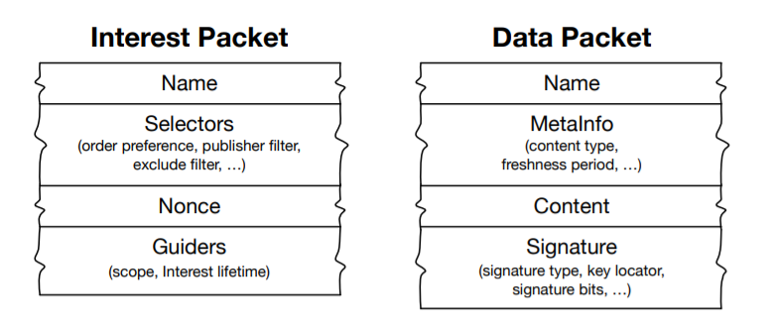
\includegraphics[width=\linewidth]{figures/packet.png}
\color{DarkSlateGray} % DarkSlateGray color for the rest of the content

%----------------------------------------------------------------------------------------
%	MATERIALS AND METHODS
%----------------------------------------------------------------------------------------

\begin{minipage}[b]{0.35\linewidth}

\section*{NDNFit\cite{zhang2018ndnfit}}
\par
	\begin{itemize}
		\item A set of \textbf{health management} applications run on NDN:
		\begin{itemize}
			\item Data storage unit(DSU);
			\item Data visualization unit(DVU);
			\item Data processing unit(DPV);
			\item Identity manager;
			\item User applications.
		\end{itemize}
		\item Different namespace for each application and user;
		\item Identity manager manages all the identities.
	\end{itemize}
\par
\end{minipage}
\begin{minipage}[b]{0.64\linewidth}
	\includegraphics[width=\linewidth]{figures/NDNfit.png}
\end{minipage}

\section*{NDN Certificate management protocol(NDNCERT)\cite{zhang2017ndncert}}
\begin{itemize}
	\item A protocol that allows auto certificate managerment;
	\item Identity will request certificate from Certificate Authority(CA);
	\item NDNCERT will be placed in identity manager;
	\item Once the certificate is acquired, it will be used to manage that namespace.
\end{itemize}

%----------------------------------------------------------------------------------------
%	OBJECTIVES
%----------------------------------------------------------------------------------------

\section*{Main Objectives}

\begin{enumerate}
\item \textbf{Use NDNCERT to write identity manager to update NDNFit;}
\item \textbf{Explore NDN development on Android and provide experience for other applications;}
\end{enumerate}

%----------------------------------------------------------------------------------------
%	RESULTS 
%----------------------------------------------------------------------------------------

\section*{Result}
\begin{itemize}
	\item Our identity manager has a new UI
	\item Following the steps the user can create a new certificate
	\item At the first time NDNFit is started, a certificate will be distributed by identity manager
\end{itemize}

\begin{minipage}[b]{0.57\linewidth}
	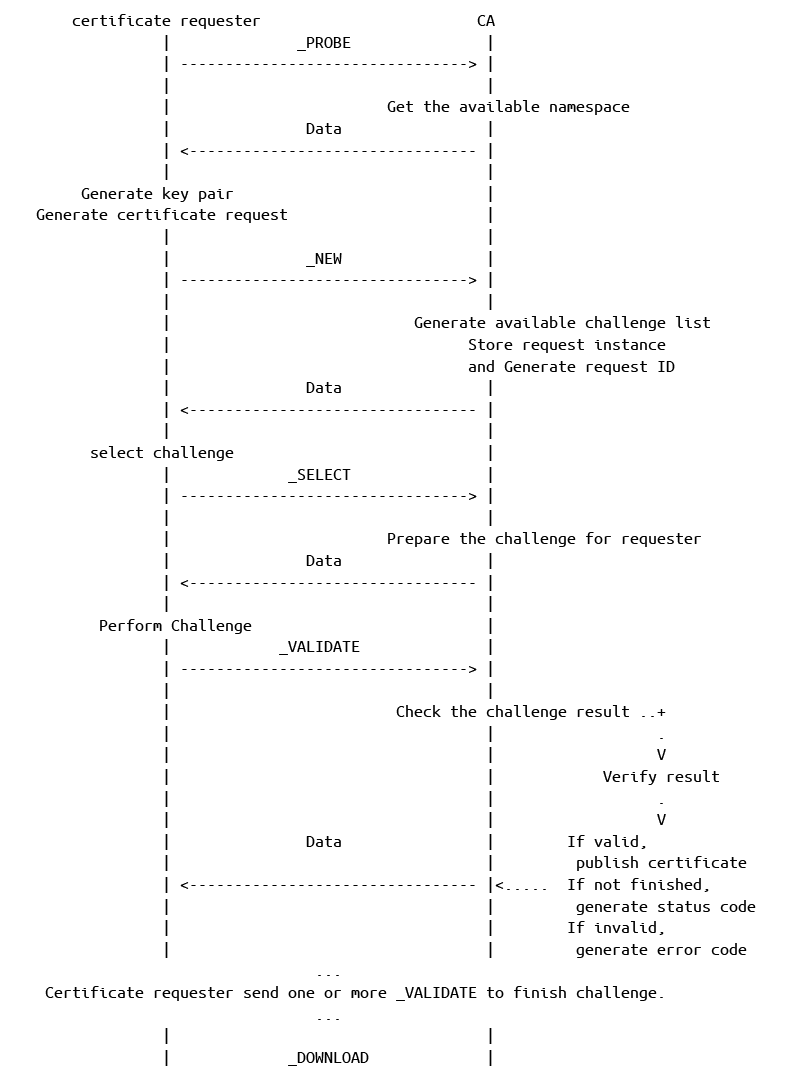
\includegraphics[width=\linewidth]{figures/protocol.png}
\end{minipage}
\begin{minipage}[b]{0.43\linewidth}
	\centering
	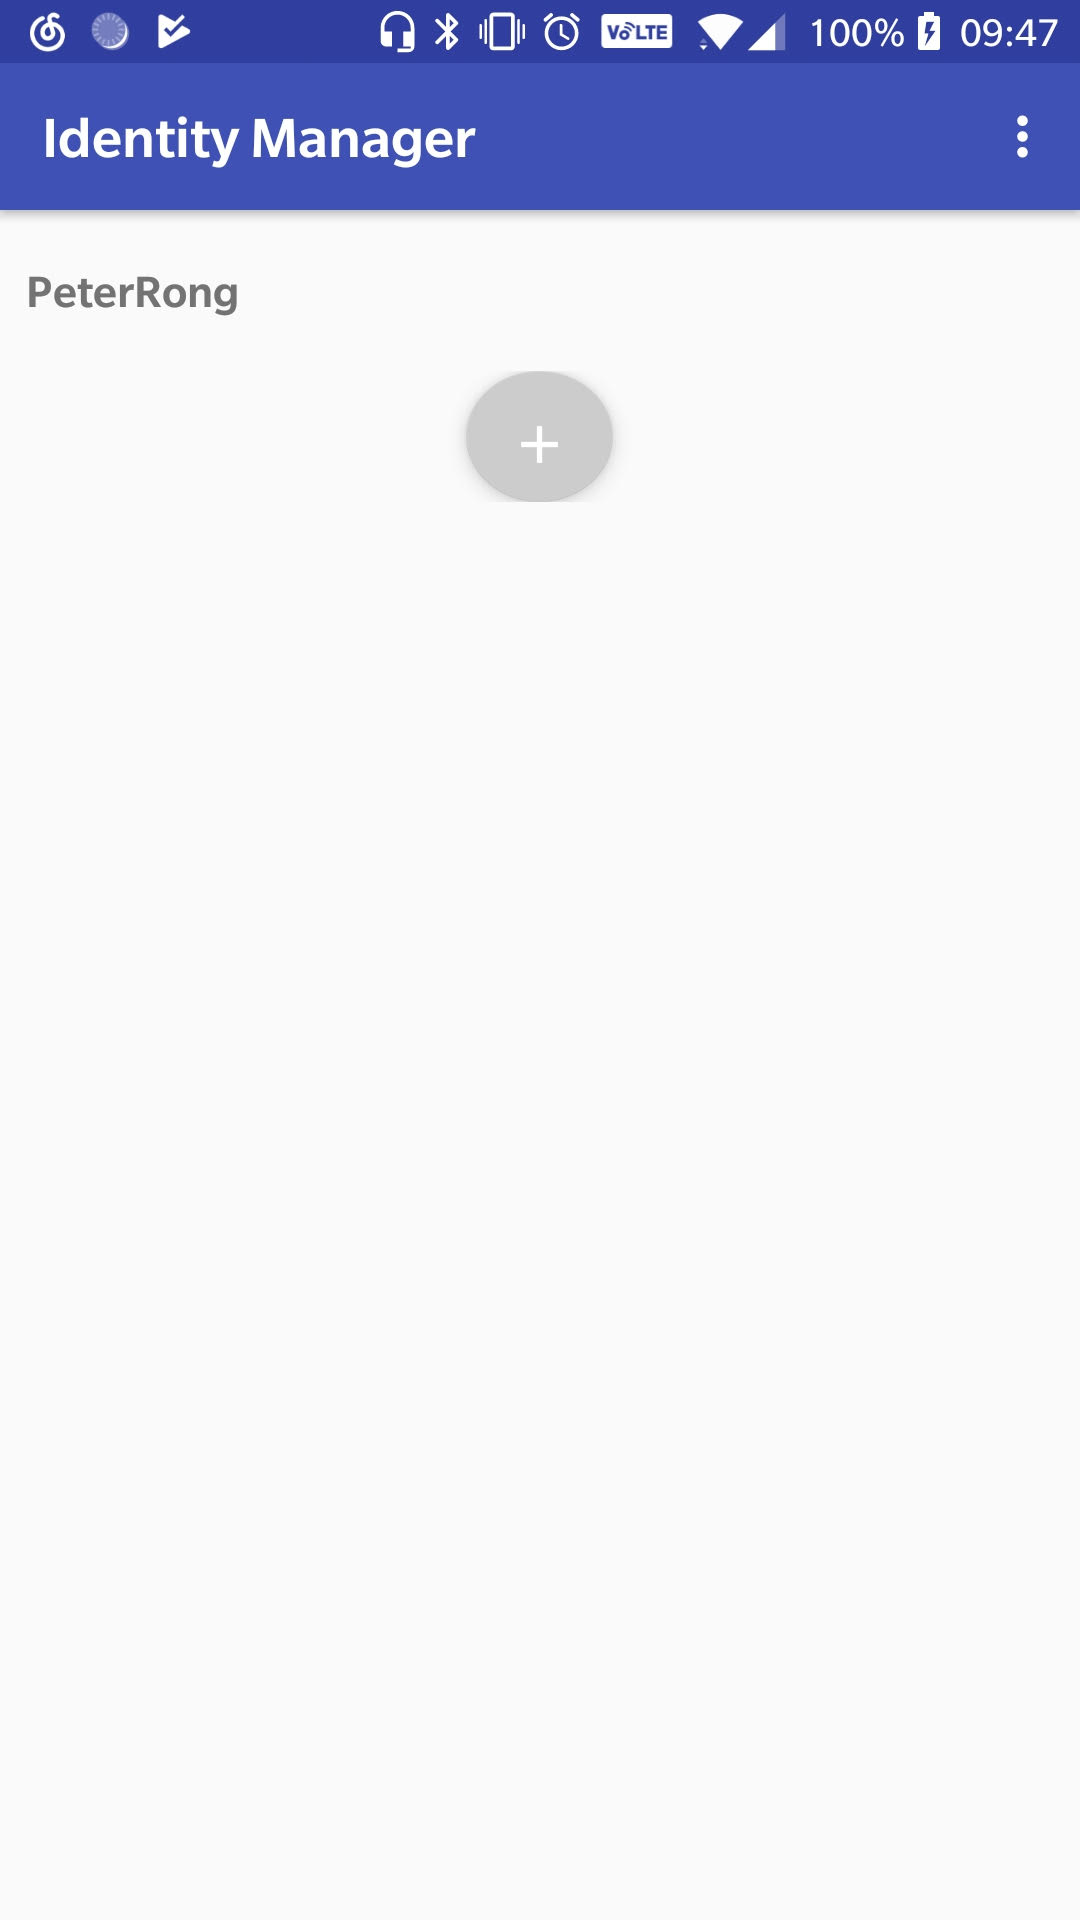
\includegraphics[width=\linewidth]{figures/main-activity.jpg}
\end{minipage}

\begin{center}
	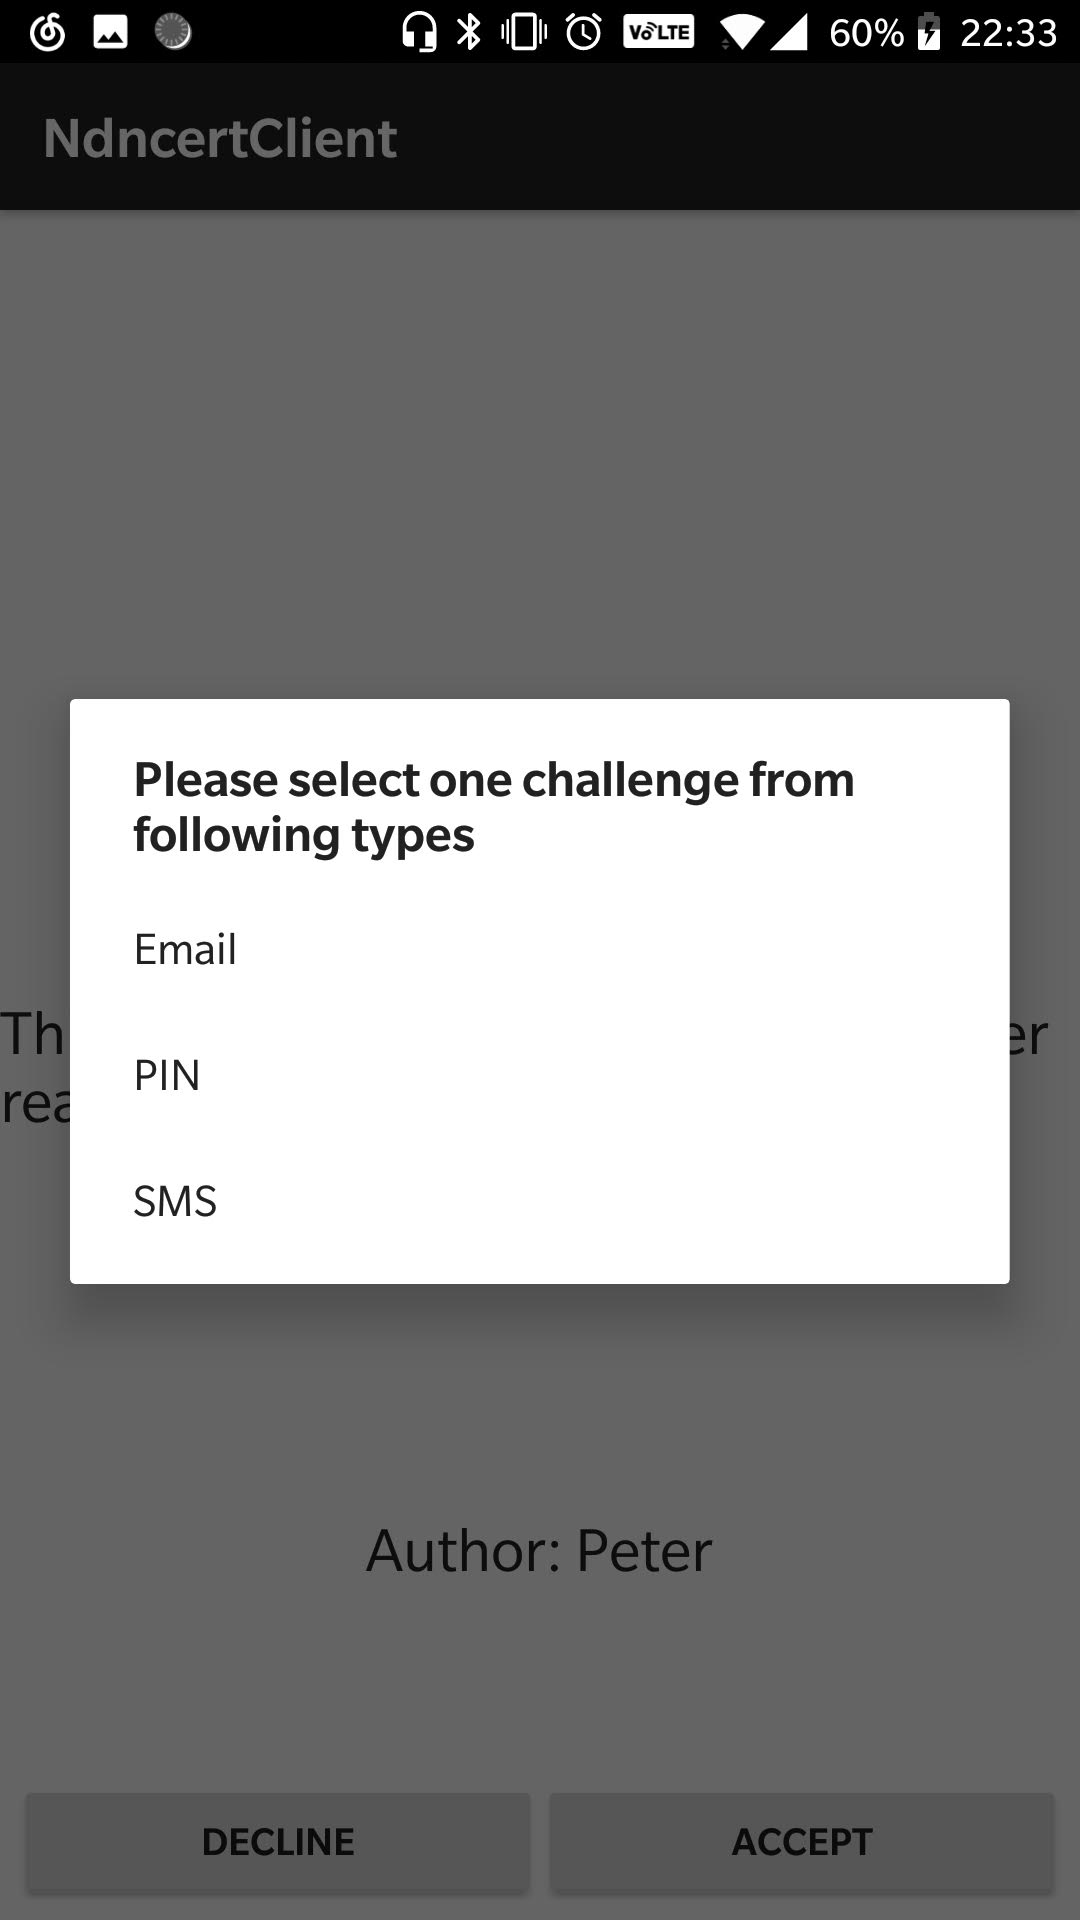
\includegraphics[width=0.27\linewidth]{figures/select.jpg}
	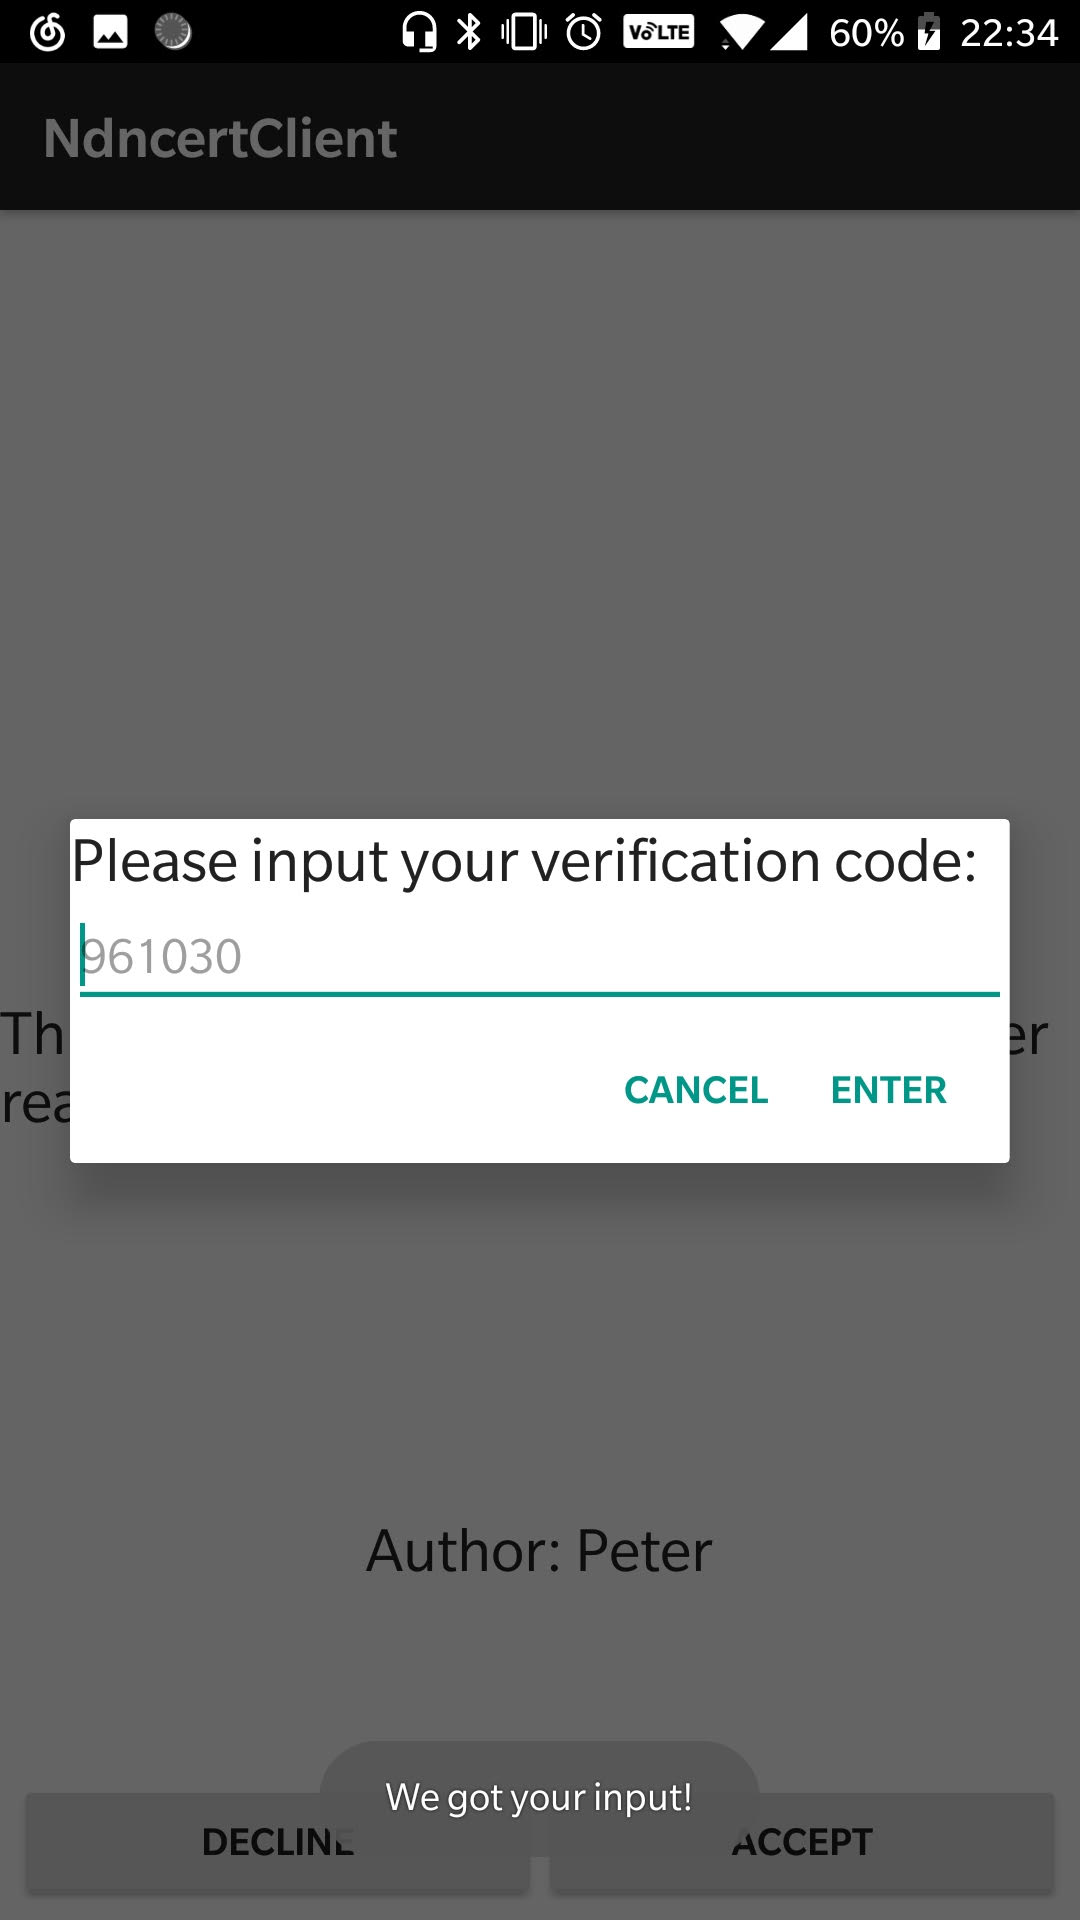
\includegraphics[width=0.27\linewidth]{figures/validate.jpg}
	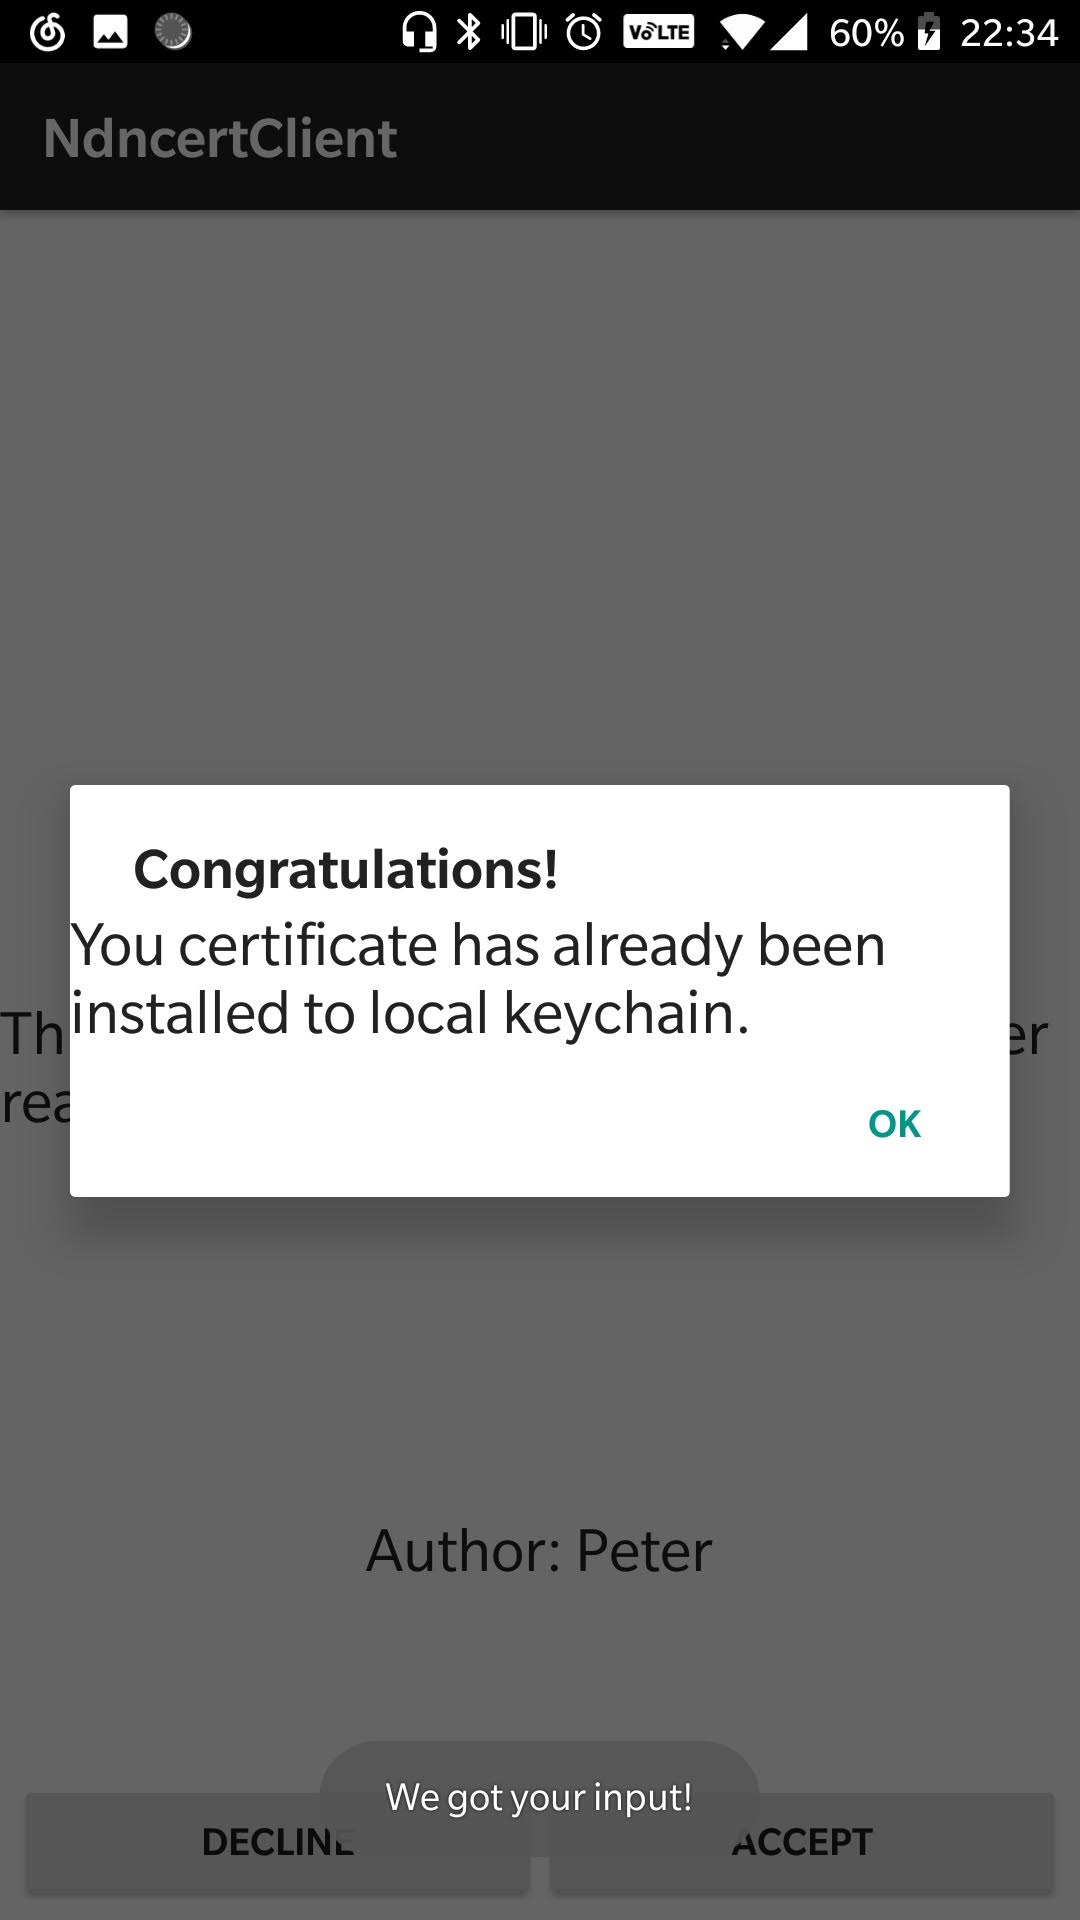
\includegraphics[width=0.27\linewidth]{figures/download.jpg}
\end{center}
%----------------------------------------------------------------------------------------
%	CONCLUSIONS
%----------------------------------------------------------------------------------------

%\color{SaddleBrown} % SaddleBrown color for the conclusions to make them stand out

%\section*{Conclusions}

%\color{DarkSlateGray} % Set the color back to DarkSlateGray for the rest of the content

%----------------------------------------------------------------------------------------
%	FORTHCOMING RESEARCH
%----------------------------------------------------------------------------------------

\section*{Future Work}

\par 
	Identity manager is about to be functional, and there are more details that can be added, including:
	\begin{itemize}
		\item identity deleting, 
		\item collision handling when identities have same name,
		\item certificate distribute when requested by other app.
	\end{itemize} 

%----------------------------------------------------------------------------------------
%	REFERENCES
%----------------------------------------------------------------------------------------

\nocite{*} % Print all references regardless of whether they were cited in the poster or not
\bibliographystyle{plain} % Plain referencing style
\bibliography{reference}
%----------------------------------------------------------------------------------------
%	ACKNOWLEDGEMENTS
%----------------------------------------------------------------------------------------

%\section*{Acknowledgments}

%\par
%	\footnotesize{We would like to thank the following people for their help:}
%	\footnotesize{
%		Lixia Zhang, Arthi Padmanabhan, Zhiyi Zhang and Alex Afanasyev. 
%		Ren Sun and CSST for providing such great opportunity.
%	}
%----------------------------------------------------------------------------------------

\end{multicols}
\end{document}